\section{Experimental results}

\begin{table}[!ht]
    \centering
    \caption{Execution time of the sequential and parallel algorithms for different matrices sizes and number of processors $P$.}
    \begin{subtable}{.45\linewidth}
        \centering
        \caption{$\textbf{A}$ \& $\textbf{B}$ of size 512x512}
        \begin{tabular}{r|r|r}
            \textbf{P} & \textbf{T\_comm} & \textbf{T\_comp} \\ \hline
            \textbf{Seq} & 0 & 50.003 \\ \hline
            \textbf{1} & 1.674681 & 50.461275 \\ \hline
            \textbf{2} & 11.206590 & 25.225144 \\ \hline
            \textbf{4} & 16.922512 & 12.566901 \\ \hline
            \textbf{8} & 32.924253 & 6.344639 \\ \hline
            \textbf{16} & 148.222790 & 3.223668 \\ \hline
            \textbf{32} & 174.169211 & 1.710644 \\ 
        \end{tabular}
    \end{subtable}
    \begin{subtable}{.45\linewidth}
        \centering
        \caption{$\textbf{A}$ \& $\textbf{B}$ of size 1024x1024}
        \begin{tabular}{r|r|r}
            \textbf{P} & \textbf{T\_comm} & \textbf{T\_comp} \\ \hline
            \textbf{Seq} & 0 & 388.730 \\ \hline
            \textbf{1} & 4.030184 & 387.597033 \\ \hline
            \textbf{2} & 19.815538 & 195.856201 \\ \hline
            \textbf{4} & 32.914310 & 101.572801 \\ \hline
            \textbf{8} & 51.866337 & 60.452539 \\ \hline
            \textbf{16} & 199.891284 & 38.215937 \\ \hline
            \textbf{32} & 300.292535 & 12.898068 \\ 
        \end{tabular}
    
    \end{subtable}
    \begin{subtable}{.45\linewidth}
        \centering
        \caption{$\textbf{A}$ \& $\textbf{B}$ of size 2048x2048}
        \begin{tabular}{r|r|r}
            \textbf{P} & \textbf{T\_comm} & \textbf{T\_comp} \\ \hline
            \textbf{Seq} & 0 & 3768.356 \\ \hline
            \textbf{1} & 13.511889 & 3819.322627 \\ \hline
            \textbf{2} & 70.904731 & 2941.665213 \\ \hline
            \textbf{4} & 67.533221 & 1335.798456 \\ \hline
            \textbf{8} & 138.074651 & 707.863888 \\ \hline
            \textbf{16} & 123.805203 & 338.441502 \\ \hline
            \textbf{32} & 275.721030 & 139.956284 \\ 
        \end{tabular}
    
    \end{subtable}
    \begin{subtable}{.45\linewidth}
        \centering
        \caption{$\textbf{A}$ \& $\textbf{B}$ of size 4096x4096}
        \begin{tabular}{r|r|r}
            \textbf{P} & \textbf{T\_comm} & \textbf{T\_comp} \\ \hline
            \textbf{Seq} & 0 & 50192.182 \\ \hline
            \textbf{1} & 54.562895 & 51104.039326 \\ \hline
            \textbf{2} & 114.210136 & 25177.496365 \\ \hline
            \textbf{4} & 251.198126 & 11896.659449 \\ \hline
            \textbf{8} & 406.719612 & 6237.871031 \\ \hline
            \textbf{16} & 244.012867 & 3085.359583 \\ \hline
            \textbf{32} & 474.394116 & 1654.710260 \\ 
        \end{tabular}
    
    \end{subtable}
    
    \label{tab:results}
\end{table}

In the experimental phase, we utilized the CAPRI \cite{1} platform to run the sequential and parallel algorithms through the SLURM scheduler. In particular, the C code has been compiled using the \textit{-O3} flag for both algorithms and compilers \textit{mpicc} and \textit{gcc} for the parallel and sequential algorithm respectively.

For simplicity of analysis, we decided to run the algorithms with square matrices of size power of 2 on powers of 2 of processors $P$; in particular the matrices are arbitrarily initialized with integers chosen uniformly at random in the range $[-99, 99]$, since the focus of this work is on the algorithms implementation and analysis.

Additionally, for each combination of sizes and number of processors, we run the algorithms a total of 5 times and take the averages as the final data. Table \ref{tab:results} reports the average results of our runs; additionally, the data for each run is also available in the repository.

As an important note, all the measurements were done on the minimal set of relevant operations, this means that from the computed times we excluded all the initialization operations, e.g. the allocation of space for $\textbf{A}$,$\textbf{B}$ and $\textbf{C}$, as well as the construction of the auxiliary data structures.

\subsection{Time performance}

Let us now consider the comparison between time performance of the sequential algorithm and the parallel algorithm, as presented in Figure \ref{fig:time_size}.

\begin{figure}[hb!]
    \centering
    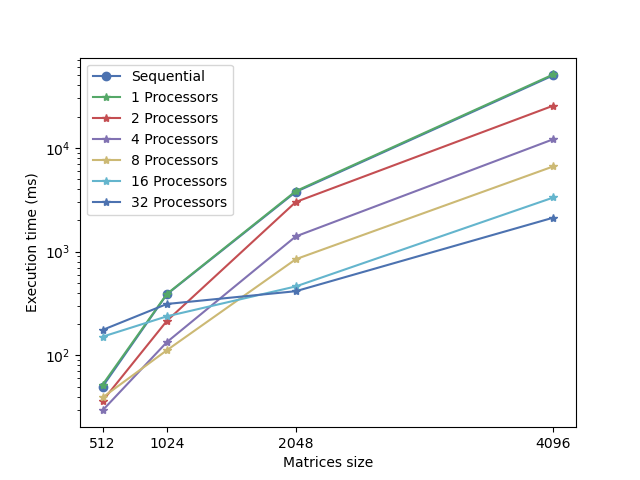
\includegraphics[width=0.8\linewidth]{figures/time_size.png}
    \caption{Time performance over matrix sizes of the sequential algorithm and parallel algorithm on a different number $P$ of processors.}
    \label{fig:time_size}
\end{figure}

As expected, we observe the well-known trade-off between computation time and communication time for higher numbers of processors characteristic to parallel algorithms: for small matrices, the communication requirements overshadow by a significant margin the gain in computation time, while for bigger matrices the distribution of the computation across many processors enables a big enough gain to greatly compensate for any time spent communicating. 
For example, from Table \ref{tab:results} we can see that for $P \ge 16$ and $M=N=O < 2048$ the communication time required to spread and gather data across this many processors takes a temporal toll that is greatly bigger than the computation time of the distributed matrix multiplication.

\begin{figure}[hb!]
    \centering
    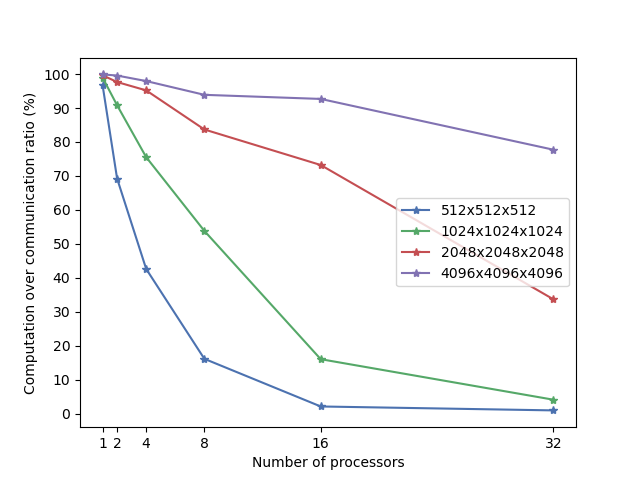
\includegraphics[width=0.8\linewidth]{figures/comp_over_comm.png}
    \caption{Computation over communication ratio on $P$ processors for the parallel algorithm, computed as $T_{\text{comp}}^p/T_{\text{total}}^p.$}
    \label{fig:compcomm}
\end{figure}

Considering also Figure \ref{fig:compcomm}, we can observe that for small matrices and high number of processors, the computation over communication ratio is particularly low, indicating that most of the time is spent on broadcasting $\textbf{B}$, scattering $\textbf{A}$ and gathering $\textbf{C}$ over actually computing the value of $\textbf{C}$; obviously this is an indication of "over-parallelization", reinforcing the well-known fact that the number of processors used should be adjusted to the size of the problem (as well as adapted to the specifics of the system used, since each network topology may be more or less susceptible to higher degrees of parallelization).
On a side note, Figure \ref{fig:compcomm} also shows the fact that the more processors we have, the higher the percentage of time spent on communicating gets for any size.

Additionally, figures like Figure \ref{fig:time_size} allow us to get an idea on the ideal number of processors to assign based on the sizes of the matrices; as mentioned earlier, a throughout analysis on the computation time is complex since it depends on both the network topology and the system load, and thus we need to rely on empirical observations to select the ideal number of processors for matrix multiplications of specific sizes.

\subsection{Speed up and scalability}

An interesting metric to consider is also the speed-up $S(P)$ provided by the parallelization process, computed as $S(P) = T_{\text{seq}}/T_{\text{parallel}}(P)$.

\begin{figure}[ht!]
    \centering
    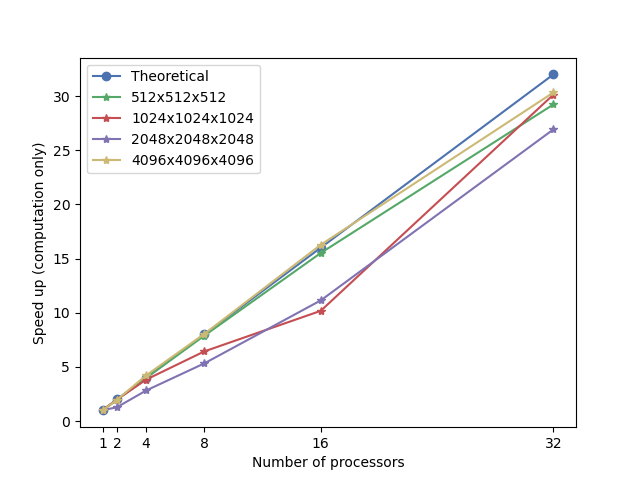
\includegraphics[width=0.8\linewidth]{figures/speedup_comp.png}
    \caption{Speed-up of parallel computation over sequential computation, computed as $S(P) = T_{\text{seq}}/T_{\text{comp}}(P)$. The theoretical speed-up refers to the speed-up theoretically obtainable by assuming the communication time to be negligible.}
    \label{fig:speedup_comp}
\end{figure}

As we mentioned in Section \ref{ssec:pperform}, the theoretical speed-up on the computation-only time provided by the parallelized algorithm is expected to be $S(P) = \Theta(P)$, and indeed Figure \ref{fig:speedup_comp} proves this bound.

\begin{figure}[hb!]
    \centering
    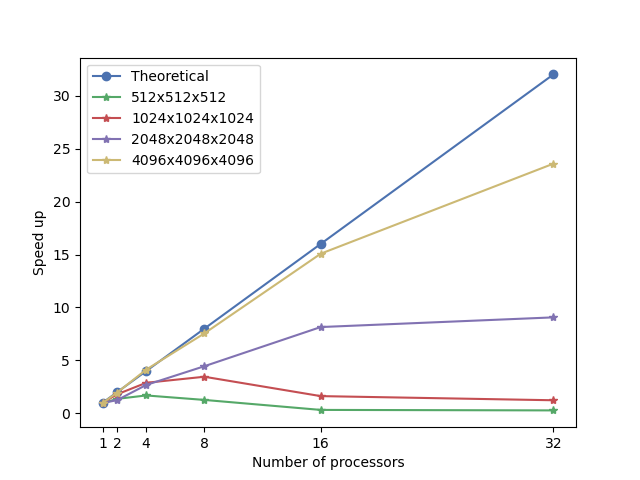
\includegraphics[width=0.8\linewidth]{figures/speedup.png}
    \caption{Speed-up of parallel algorithm over sequential one, computed as $S(P) = T_{\text{seq}}/T_{\text{parallel}}(P)$. The theoretical speed-up refers to the speed-up theoretically obtainable by assuming the communication time to be negligible.}
    \label{fig:speedup}
\end{figure}

However, the situation becomes again more complex as soon as we also factor in the communication time: Figure \ref{fig:speedup} shows the speed-up computed on $T_{\text{parallel}}(P)$ and highlights again how an excessive number of processors assigned overshadows the computation speed-up by an excessively dominating communication time. In particular, we can observe how the bigger the matrices are and the closer we are to the theoretical speed-up as the number of processor increases; additionally, we can also appreciate the fall-off caused by an over-increasing number of processors on smaller sizes of matrices.

Essentially, it is straightforward to see that on the CAPRI infrastructure our parallel algorithm is not scalable, since our experiments show how the speed-up factor decreases as the number of processors increases too much, even going into values lower than 1 (i.e. negative performance impact compared to the sequential algorithm) for the smaller matrices.
On a final note, it is worth to point out that, theoretically speaking, other network topologies may be able to scale better, but in practice such systems would be unfeasible and thus a certain degree of performance deterioration is likely to always be observed as the number of processors increases too much over the sizes of the matrices.